%!TEX program = xelatex
%==============================================================================
%  初中英语词汇量快速定级测试单（人教版 2024 新版 · 成都适用）
%  升级版 v2.0 —— LaTeX 源码
%------------------------------------------------------------------------------
%  【编译方式】XeLaTeX 连续编译两次（或 latexmk -xelatex 本文件.tex）
%      xelatex 初中英语词汇量快速定级测试单_升级版v2.tex
%      xelatex 初中英语词汇量快速定级测试单_升级版v2.tex
%  【依赖环境】TeX Live 2023 及以上 / MiKTeX 完整安装，含以下宏包：
%      ctex, tcolorbox, tikz, tabularx, booktabs, makecell, enumitem,
%      fancyhdr, lastpage, needspace, xcolor, hyperref
%  【字体说明】默认调用 Windows 系统字体（宋体 SimSun / 黑体 SimHei）。
%      在 macOS 上编译：把下一行的 fontset=windows 改为 fontset=macnew；
%      在 Linux 上编译：改为 fontset=fandol 或 fontset=ubuntu。
%  【使用许可】可自由复印用于课堂教学；修改后请保留本段说明。
%==============================================================================
\documentclass[UTF8, fontset=windows, a4paper, zihao=5]{ctexart}

%------------------------------ 宏包与页面 ------------------------------------
\usepackage[table]{xcolor}
\usepackage[a4paper, left=1.7cm, right=1.7cm, top=2.0cm, bottom=1.9cm,
            headheight=19pt, headsep=7pt, footskip=13pt, includefoot]{geometry}
\usepackage{tcolorbox}
\tcbuselibrary{skins, breakable}
\usepackage{tikz}
\usepackage{tabularx}
\usepackage{booktabs}
\usepackage{makecell}
\usepackage{enumitem}
\usepackage{amsmath, amssymb}
\usepackage{fancyhdr}
\usepackage{lastpage}
\usepackage{needspace}
\usepackage[hidelinks]{hyperref}

%------------------------------ 配色 ------------------------------------------
\definecolor{main}{HTML}{134B70}    % 主色：深蓝
\definecolor{main2}{HTML}{2E7DA8}   % 辅色：亮蓝
\definecolor{accent}{HTML}{C0553F}  % 强调色：砖红
\definecolor{graytext}{HTML}{5B6B7B}
\definecolor{line}{HTML}{C3D2DE}
\definecolor{paper}{HTML}{F3F7FA}
\definecolor{lvA}{HTML}{4C8CB5}     % Level 1
\definecolor{lvB}{HTML}{3D7CA3}     % Level 2
\definecolor{lvC}{HTML}{2E6C94}     % Level 3
\definecolor{lvD}{HTML}{1F5C82}     % Level 4
\definecolor{lvE}{HTML}{12496E}     % Level 5

%------------------------------ 版式设置 --------------------------------------
\linespread{1.16}
\setlength{\parindent}{0pt}
\setlength{\parskip}{0pt}
\setlength{\tabcolsep}{4pt}
\renewcommand{\arraystretch}{1.15}
\setlist[itemize]{leftmargin=1.6em, itemsep=0.25ex, topsep=0.3ex, parsep=0pt}
\setlist[enumerate]{leftmargin=2.3em, itemsep=0.35ex, topsep=0.3ex, parsep=0pt}

%------------------------------ 页眉页脚 --------------------------------------
\pagestyle{fancy}
\fancyhf{}
\renewcommand{\headrulewidth}{0.4pt}
\renewcommand{\headrule}{\hbox to\headwidth{\color{line}\leaders\hrule height \headrulewidth\hfill}}
\fancyhead[L]{\footnotesize\color{graytext}初中英语词汇量快速定级测试单}
\fancyhead[R]{\footnotesize\color{graytext}人教版 2024 新版 · 成都适用 · 升级版 v2.0}
\fancyfoot[L]{\footnotesize\color{graytext}第 \thepage\ 页 / 共 \pageref{LastPage} 页}
\fancyfoot[C]{\footnotesize\color{graytext}本单可复印用于班级测试}
\fancyfoot[R]{\footnotesize\color{graytext}建议每学期复测一次}

%------------------------------ PDF 元信息 ------------------------------------
\hypersetup{
  pdftitle={初中英语词汇量快速定级测试单（升级版 v2.0）},
  pdfsubject={人教版 2024 新版 · 成都适用 · 初中英语词汇量快速定级},
  pdfkeywords={初中英语, 词汇量, 定级测试, 人教版2024, 成都, 初二, 初三}
}

%------------------------------ 自定义命令 ------------------------------------
% 填空横线：#1 为长度（默认 2.3cm）
\newcommand{\fillin}[1][2.3cm]{\rule[-0.45ex]{#1}{0.5pt}}

% 空白勾选框（TikZ 绘制，打印清晰、大小统一）
\newcommand{\cb}{%
  \tikz[baseline=-0.55ex]{\draw[draw=main!60, line width=0.5pt, fill=white]
    (0,0) rectangle (9.5pt,9.5pt);}}

% 已勾选框（示范用）：方框 + 砖红对勾
\newcommand{\cbt}{%
  \tikz[baseline=-0.55ex]{%
    \draw[draw=main!60, line width=0.5pt, fill=white] (0,0) rectangle (9.5pt,9.5pt);
    \draw[accent, line width=0.9pt, line cap=round]
      (1.6pt,5pt) -- (4pt,2.1pt) -- (8.2pt,8pt);}}

% 词表单元格：勾选框 + 序号 + 单词（方框在词前，纵向对齐更整齐）
\newcommand{\wordcell}[2]{%
  \cb\hspace{0.55em}%
  \makebox[0.72cm][r]{\textcolor{graytext}{\small #1.}}%
  \hspace{0.25em}#2}

% 答案单元格：序号 + 单词 + 词性 + 中文释义
\newcommand{\anscell}[4]{%
  \makecell[l]{\textbf{\textcolor{main!85}{#1.}}\ \textbf{#2}\\%
    {\footnotesize\itshape\textcolor{graytext}{#3}}\hspace{0.25em}{\footnotesize #4}}}

% 一级标题：色块编号 + 主标题 + 副标题 + 分隔线
\newcommand{\Section}[3]{%
  \par\addvspace{1.5ex plus .3ex}%
  \needspace{5\baselineskip}%
  \noindent
  {\colorbox{main}{\textcolor{white}{\heiti\small\strut #1}}}%
  \hspace{0.8em}{\heiti\Large\textcolor{main}{#2}}%
  \hspace{0.6em}{\heiti\small\textcolor{main2}{#3}}\par
  \vspace{0.6ex}%
  \noindent{\textcolor{main!30}{\rule{\linewidth}{1pt}}}\par
  \addvspace{0.9ex}%
}

% 级别色带：整行标题条（左侧级别名称，右侧教材与累计词量）
\newcommand{\levelband}[3]{%
  \par\addvspace{0.6ex}\needspace{8\baselineskip}%
  \noindent\colorbox{#1}{%
    \parbox{\dimexpr\linewidth-2\fboxsep\relax}{%
      \textcolor{white}{\heiti\small\strut #2}\hfill
      \textcolor{white!88}{\mdseries\footnotesize #3}\strut}}\par
  \vspace{0.4ex}%
}

% 答案区级别小标题
\newcommand{\ansband}[2]{%
  \par\addvspace{0.5ex}\noindent
  {\textcolor{#1}{\rule[-0.15ex]{4pt}{1.45ex}}}\hspace{0.6em}%
  {\heiti\small\textcolor{#1}{#2}}\par\vspace{0.25ex}%
}

% 学生用词表（5 列 × 4 行，共 20 词）
\newenvironment{wordgrid}{%
  \par\noindent
  \small
  \renewcommand{\arraystretch}{1.3}%
  \tabularx{\linewidth}{@{}>{\raggedright\arraybackslash}X
      >{\raggedright\arraybackslash}X>{\raggedright\arraybackslash}X
      >{\raggedright\arraybackslash}X>{\raggedright\arraybackslash}X@{}}%
}{%
  \endtabularx\par\vspace{0.1ex}%
  {\footnotesize\color{graytext}\noindent
   教师抽查：本级别任选 2 个已勾词，让学生说出中文意思\hfill
   \cb\,全对\quad \cb\,错 1\quad \cb\,错 2\par}%
  \vspace{0.7ex}%
}

% 教师用答案表（4 列 × 5 行，与词表顺序一一对应）
\newenvironment{ansgrid}{%
  \par\noindent\small
  \renewcommand{\arraystretch}{1.08}%
  \tabularx{\linewidth}{@{}>{\raggedright\arraybackslash}X
      >{\raggedright\arraybackslash}X>{\raggedright\arraybackslash}X
      >{\raggedright\arraybackslash}X>{\raggedright\arraybackslash}X@{}}%
}{%
  \endtabularx\par\vspace{0.35ex}%
}

% 轻量信息框样式
\tcbset{
  softbox/.style={enhanced, colback=paper, colframe=line, boxrule=0.5pt,
    arc=1.2mm, left=3mm, right=3mm, top=2mm, bottom=2mm},
  card/.style={enhanced, breakable, colback=white, colframe=main,
    boxrule=0.8pt, arc=3mm, left=4mm, right=4mm, top=3mm, bottom=3mm,
    fonttitle=\heiti\small, colbacktitle=main, coltitle=white,
    toptitle=1.3mm, bottomtitle=1.3mm, titlerule=0pt},
}

%==============================================================================
\begin{document}

%------------------------------ 标题区 ----------------------------------------
\begin{tcolorbox}[enhanced, colback=main, colframe=main, arc=2.5mm,
  boxrule=0pt, left=6mm, right=6mm, top=5.5mm, bottom=5.5mm]
\centering
{\color{white}\heiti\fontsize{23}{28}\selectfont
 初中英语词汇量快速定级测试单}\par
\vspace{1.4mm}
{\color{accent!85}\rule{2.6cm}{1.6pt}}\par
\vspace{1.4mm}
{\color{white!92}\heiti\normalsize
 人教版《英语》（2024 新版）· 成都适用 · 初二／初三}\par
\vspace{0.9mm}
{\color{white!72}\footnotesize
 5 级 × 20 词 ＝ 100 词　｜　5–8 分钟测完　｜　当场定级　｜　升级版 v2.0}\par
\end{tcolorbox}

%------------------------------ 学生信息 --------------------------------------
\vspace{1.2ex}
\begin{tcolorbox}[softbox]
{\small
\noindent
\textbf{姓名}\ \fillin[2.4cm]\hfill
\textbf{班级}\ \fillin[2.4cm]\hfill
\textbf{学校}\ \fillin[3.6cm]\par\vspace{1.5mm}
\noindent
\textbf{日期}\ \fillin[2.4cm]\hfill
\textbf{开始时间}\ \fillin[1.9cm]\hfill
\textbf{结束时间}\ \fillin[1.9cm]\hfill
\textbf{实际用时}\ \fillin[1.9cm]
}
\end{tcolorbox}

%------------------------------ 一、测试说明 ----------------------------------
\Section{一}{测试说明}{学生用}\label{sec:info}
\begin{enumerate}[label=\textcolor{main}{\bfseries\arabic*.}]
\item 本单共 5 个级别、100 个单词，全部抽样自人教版《英语》（2024 新版）
  七年级上册至九年级各册单词表（成都市现行教材版本）。
\item 从 Level 1 开始逐词快速浏览：能说出中文意思的词，在词前的小方框中打
  \textcolor{accent}{$\checkmark$}；说不出或拿不准的，直接跳过——不猜、不查、不讨论。
\item 全程约 5–8 分钟，凭第一反应作答；做不完不影响定级，宁可少勾，不要多勾。
\item 一词多义时，说出任一个常见义项即可；只认得词形、说不出意思，不算认识。
\item 完成后，老师／家长会从每个级别随机抽 2 个已勾词，请你口头说中文意思
  （答案表见第 \pageref{sec:answers} 页），抽查不一致的词按“不认识”计。
\item 适用范围：初二、初三；初一期末可只做 Level 1–2 自测（未做的级别按 0 计）。
  不适用于小学及高中。
\end{enumerate}

\begin{tcolorbox}[softbox]
{\small
\textbf{勾选示例}\quad
\cbt\ \textcolor{graytext}{apple}\quad
{\footnotesize\color{graytext}（认识 $\to$ 打 $\checkmark$）}\hspace{1.6em}
\cb\ \textcolor{graytext}{timetable}\quad
{\footnotesize\color{graytext}（不认识 $\to$ 留空）}\par\vspace{0.6mm}
{\footnotesize\color{graytext}
 提示：示例词不计入测试；不确定的词请不要“试探性”勾选——留空最能反映真实水平。}
}
\end{tcolorbox}

%------------------------------ 本单结构 --------------------------------------
\vspace{0.6ex}
\begin{tcolorbox}[softbox]
{\small\heiti\color{main}本单结构一览\par}
\vspace{0.4ex}
\begin{tabularx}{\linewidth}{@{}>{\centering\arraybackslash}p{2.0cm}
    >{\raggedright\arraybackslash}p{3.6cm}
    >{\centering\arraybackslash}p{2.2cm}
    >{\raggedright\arraybackslash}X@{}}
\arrayrulecolor{line}
\toprule[0.5pt]
{\footnotesize 页码} & {\footnotesize 板块} & {\footnotesize 使用者} & {\footnotesize 内容}\\
\midrule
{\footnotesize 第 \pageref{sec:info} 页} & {\footnotesize 测试说明} & {\footnotesize 学生}
  & {\footnotesize 读规则、填个人信息}\\
{\footnotesize 第 \pageref{sec:words} 页} & {\footnotesize 五级词表} & {\footnotesize 学生}
  & {\footnotesize 5–8 分钟逐词勾选}\\
{\footnotesize 第 \pageref{sec:score} 页} & {\footnotesize 评分与定级} & {\footnotesize 教师}
  & {\footnotesize 判级、估算词汇量}\\
{\footnotesize 第 \pageref{sec:answers} 页} & {\footnotesize 抽查答案表} & {\footnotesize 教师}
  & {\footnotesize 口头抽查核对}\\
{\footnotesize 第 \pageref{sec:levels} 页} & {\footnotesize 水平对照与复测} & {\footnotesize 教师／家长}
  & {\footnotesize 看水平、定回补计划}\\
{\footnotesize 第 \pageref{sec:result} 页} & {\footnotesize 定级结果卡} & {\footnotesize 师生}
  & {\footnotesize 填写存档、追踪进步}\\
\bottomrule[0.5pt]
\end{tabularx}
\end{tcolorbox}

%------------------------------ 测试流程 --------------------------------------
\vspace{0.6ex}
\begin{tcolorbox}[softbox]
{\small\heiti\color{main}测试流程（教师 5 分钟上手）\par}
\small
\begin{enumerate}[label=\textcolor{main}{\bfseries\arabic*.},
  leftmargin=2.0em, itemsep=0.15ex, topsep=0.4ex]
\item \textbf{打印}：A4 双面打印；第 1–2 页交学生，第 3–5 页教师留存，
  第 6 页结果卡填写后交老师存档。
\item \textbf{施测}：发单、读规则、计时 5–8 分钟；学生逐词打勾，不许查词、不许讨论。
\item \textbf{计分}：按第三部分逐级数勾，判定每级“通过／边缘／未过”。
\item \textbf{定级}：用精确法（或速查表）估算词汇量，填写结果卡。
\item \textbf{抽查与回补}：每级抽 2 词口头复核；按第五部分锁定回补级别，安排复测。
\end{enumerate}
\end{tcolorbox}

\clearpage
%==============================================================================
%  二、五个级别词表
%==============================================================================
\Section{二}{五个级别词表}{学生用 · 逐级勾选}\label{sec:words}
{\footnotesize\color{graytext}
 五个级别由易到难，累计词汇量约 450 $\to$ 2400 词。每级 20 词，规则同上；
 若某一级别几乎一个都不认识，可停笔，其余级别按 0 计，
 并在结果卡上记“止于第 X 级”。}
\vspace{0.5ex}

%------------------------------ Level 1 ---------------------------------------
\levelband{lvA}{Level 1　起步级}{对应教材：七年级上册（本级约 450 词）\quad 累计约 450 词\quad $\bullet\circ\circ\circ\circ$}
\begin{wordgrid}
\wordcell{1}{grade} & \wordcell{2}{classmate} & \wordcell{3}{mistake} & \wordcell{4}{country} & \wordcell{5}{twin}\\
\wordcell{6}{handsome} & \wordcell{7}{together} & \wordcell{8}{building} & \wordcell{9}{important} & \wordcell{10}{notice}\\
\wordcell{11}{useful} & \wordcell{12}{exciting} & \wordcell{13}{remember} & \wordcell{14}{future} & \wordcell{15}{join}\\
\wordcell{16}{choose} & \wordcell{17}{interested} & \wordcell{18}{shower} & \wordcell{19}{routine} & \wordcell{20}{celebrate}\\
\end{wordgrid}

%------------------------------ Level 2 ---------------------------------------
\levelband{lvB}{Level 2　基础级}{对应教材：七年级下册（本级约 500 词）\quad 累计约 950 词\quad $\bullet\bullet\circ\circ\circ$}
\begin{wordgrid}
\wordcell{1}{giraffe} & \wordcell{2}{dangerous} & \wordcell{3}{forest} & \wordcell{4}{friendly} & \wordcell{5}{rule}\\
\wordcell{6}{follow} & \wordcell{7}{polite} & \wordcell{8}{respect} & \wordcell{9}{practice} & \wordcell{10}{advice}\\
\wordcell{11}{energy} & \wordcell{12}{encourage} & \wordcell{13}{progress} & \wordcell{14}{watermelon} & \wordcell{15}{menu}\\
\wordcell{16}{enough} & \wordcell{17}{station} & \wordcell{18}{weather} & \wordcell{19}{temperature} & \wordcell{20}{museum}\\
\end{wordgrid}

%------------------------------ Level 3 ---------------------------------------
\levelband{lvC}{Level 3　进阶级}{对应教材：八年级上册（本级约 500 词）\quad 累计约 1450 词\quad $\bullet\bullet\bullet\circ\circ$}
\begin{wordgrid}
\wordcell{1}{wonderful} & \wordcell{2}{bored} & \wordcell{3}{housework} & \wordcell{4}{hardly} & \wordcell{5}{percent}\\
\wordcell{6}{although} & \wordcell{7}{outgoing} & \wordcell{8}{competition} & \wordcell{9}{talented} & \wordcell{10}{necessary}\\
\wordcell{11}{comfortable} & \wordcell{12}{educational} & \wordcell{13}{expect} & \wordcell{14}{engineer} & \wordcell{15}{resolution}\\
\wordcell{16}{improve} & \wordcell{17}{environment} & \wordcell{18}{pollution} & \wordcell{19}{available} & \wordcell{20}{experience}\\
\end{wordgrid}

%------------------------------ Level 4 ---------------------------------------
\levelband{lvD}{Level 4　熟练级}{对应教材：八年级下册（本级约 450 词）\quad 累计约 1900 词\quad $\bullet\bullet\bullet\bullet\circ$}
\begin{wordgrid}
\wordcell{1}{matter} & \wordcell{2}{volunteer} & \wordcell{3}{satisfaction} & \wordcell{4}{borrow} & \wordcell{5}{provide}\\
\wordcell{6}{independence} & \wordcell{7}{argue} & \wordcell{8}{nervous} & \wordcell{9}{communicate} & \wordcell{10}{pressure}\\
\wordcell{11}{suddenly} & \wordcell{12}{remind} & \wordcell{13}{population} & \wordcell{14}{protect} & \wordcell{15}{achievement}\\
\wordcell{16}{treasure} & \wordcell{17}{technology} & \wordcell{18}{actually} & \wordcell{19}{unbelievable} & \wordcell{20}{memory}\\
\end{wordgrid}

%------------------------------ Level 5 ---------------------------------------
\levelband{lvE}{Level 5　优秀级}{对应教材：九年级＋中考冲刺（本级约 500 词）\quad 累计约 2400 词\quad $\bullet\bullet\bullet\bullet\bullet$}
\begin{wordgrid}
\wordcell{1}{government} & \wordcell{2}{support} & \wordcell{3}{product} & \wordcell{4}{digital} & \wordcell{5}{convenient}\\
\wordcell{6}{business} & \wordcell{7}{benefit} & \wordcell{8}{miracle} & \wordcell{9}{inspire} & \wordcell{10}{courage}\\
\wordcell{11}{knowledge} & \wordcell{12}{patient} & \wordcell{13}{attention} & \wordcell{14}{invent} & \wordcell{15}{allow}\\
\wordcell{16}{belong} & \wordcell{17}{suppose} & \wordcell{18}{recycle} & \wordcell{19}{industry} & \wordcell{20}{responsible}\\
\end{wordgrid}

{\footnotesize\color{graytext}
 计分小提示：每级 20 词，勾选数 $\ge 16$ 为“通过”，12–15 为“边缘”，$\le 11$ 为“未过”；
 定级与词汇量估算方法见第 \pageref{sec:score} 页。}

\clearpage
%==============================================================================
%  三、评分与定级
%==============================================================================
\Section{三}{评分与定级}{教师／家长用}\label{sec:score}
{\footnotesize\color{graytext}
 逐级统计勾选数并判级，再用“精确法”或“速查表”估算词汇量，最后填写结果卡。}
\vspace{0.3ex}

\begin{center}
\begin{tabularx}{\linewidth}{@{}>{\centering\arraybackslash}X
    >{\centering\arraybackslash}X>{\centering\arraybackslash}X
    >{\centering\arraybackslash}X@{}}
\arrayrulecolor{line}
\toprule[0.6pt]
{\small\bfseries\textcolor{main}{判定}} & {\small\bfseries\textcolor{main}{通过}}
  & {\small\bfseries\textcolor{main}{边缘}} & {\small\bfseries\textcolor{main}{未过}}\\
\midrule
{\small 每级勾选数} & {\small $\ge 16$ 个} & {\small 12–15 个} & {\small $\le 11$ 个}\\
\bottomrule[0.6pt]
\end{tabularx}
\end{center}
{\footnotesize\color{graytext}每级 20 词；各级累计词量见第五部分的水平对照表。}
\vspace{0.3ex}

\begin{enumerate}[label=\textcolor{main}{\bfseries\arabic*.}]
\item \textbf{定级规则}：从 Level 1 起逐级查看，取“连续通过”的最高级为该生词汇定级。
  若 L1 未达通过，定级记作“未达 Level 1”；若最高通过级之后一级为“边缘”，
  记作“X 级边缘”（X 为最高通过级，例：L1–L3 通过、L4 边缘
  $\to$ 定级“Level 3 边缘”，对照水平表时按 Level 3 行使用）。
  停笔或未做的级别按 0 计。
\item \textbf{精确法估算词汇量}：以“第一个未达到通过标准的级别”（边缘或未过）为第 $k$ 级
  （五级全过时取 $k=5$），
  \begin{tcolorbox}[softbox, left=4mm, right=4mm, top=1.6mm, bottom=1.6mm]
  {\small
   \textbf{词汇量} $\approx$ \textbf{前 $k-1$ 级累计词量}
   ＋（\textbf{第 $k$ 级勾选数} ÷ 20）× \textbf{第 $k$ 级增量词量}}
  \end{tcolorbox}
  {\small
   \textbf{算例 A}：L1–L3 通过，L4 停测（勾 8 个）$\to$ 1450 ＋ (8 ÷ 20) × 450
   $\approx$ \textbf{1630 词}（定级 Level 3）。\par
   \textbf{算例 B}：L1 勾 19，L2 通过，L3 停测（勾 10 个）$\to$ 950 ＋ (10 ÷ 20) × 500
   ＝ \textbf{1200 词}（定级 Level 2）。\par
   五级全过：按第 5 级代入公式，约 \textbf{2300–2400 词}；勾满 20 个即 \textbf{2400 词}。}
\item \textbf{快速粗估}（不便逐级分类时）：\textbf{总勾选数 × 24 $\approx$ 词汇量}，
  抽样误差约 ±10\%。例：勾 60 个 $\approx$ 1440 词；勾 80 个 $\approx$ 1920 词。
  此法仅作粗略比较（对高级别学生会偏低），与精确法不一致时以精确法为准。
\item \textbf{期望线}：初二 $\ge$ Level 3；初三 $\ge$ Level 4；中考冲刺 $\ge$ Level 5。
  低于期望一个级别以上，建议按第五部分的“回补重点”专项补词。
\item \textbf{结果效力}：若实际用时超过 12 分钟，或抽查错误 $\ge 2$ 个，
  本次结果仅作参考，建议隔 1–2 周重测。
\end{enumerate}

%------------------------------ 定级速查表 ------------------------------------
\vspace{0.3ex}
{\small\heiti\color{main}定级与词汇量速查表}
\hspace{0.5em}{\footnotesize\color{graytext}（按定级结果直接查；精确数值用上方公式）}
\vspace{0.4ex}

\begin{tabularx}{\linewidth}{@{}>{\raggedright\arraybackslash}p{3.3cm}
    >{\raggedright\arraybackslash}p{5.4cm}
    >{\centering\arraybackslash}X@{}}
\arrayrulecolor{line}
\toprule[0.5pt]
{\footnotesize\bfseries\textcolor{main}{定级结果}}
  & {\footnotesize\bfseries\textcolor{main}{判定情形}}
  & {\footnotesize\bfseries\textcolor{main}{估算词汇量}}\\
\midrule
{\footnotesize 未达 Level 1} & {\footnotesize L1 勾选 0–15 个（含 L1 边缘）}
  & {\footnotesize 0–338}\\
{\footnotesize Level 1} & {\footnotesize L1 通过，L2 勾选 0–11 个}
  & {\footnotesize 450–725}\\
{\footnotesize Level 1 边缘} & {\footnotesize L1 通过，L2 勾选 12–15 个}
  & {\footnotesize 750–825}\\
{\footnotesize Level 2} & {\footnotesize L2 通过，L3 勾选 0–11 个}
  & {\footnotesize 950–1225}\\
{\footnotesize Level 2 边缘} & {\footnotesize L2 通过，L3 勾选 12–15 个}
  & {\footnotesize 1250–1325}\\
{\footnotesize Level 3} & {\footnotesize L3 通过，L4 勾选 0–11 个}
  & {\footnotesize 1450–1698}\\
{\footnotesize Level 3 边缘} & {\footnotesize L3 通过，L4 勾选 12–15 个}
  & {\footnotesize 1720–1788}\\
{\footnotesize Level 4} & {\footnotesize L4 通过，L5 勾选 0–11 个}
  & {\footnotesize 1900–2175}\\
{\footnotesize Level 4 边缘} & {\footnotesize L4 通过，L5 勾选 12–15 个}
  & {\footnotesize 2200–2275}\\
{\footnotesize Level 5} & {\footnotesize 五级全部通过（L5 勾选 16–20 个）}
  & {\footnotesize 2300–2400}\\
\bottomrule[0.5pt]
\end{tabularx}
\par\vspace{0.25ex}
{\footnotesize\color{graytext}
 说明：区间按“通过 = 本级勾选 16–20 个”推算；需要更精确的数值时，用上方精确法公式。
 停笔或未做的级别按 0 计；X 级边缘按 X 级行对照第五部分水平表。}

%------------------------------ 教师须知 --------------------------------------
\vspace{0.6ex}
\begin{tcolorbox}[softbox]
{\small\heiti\color{main}教师须知\par}
\small
\begin{itemize}[leftmargin=1.4em, itemsep=0.2ex, topsep=0.4ex]
\item {\bfseries 施测环境}：安静、无词典／手机／翻译笔；学生之间不讨论。
  教师只提示“开始”和“还剩 1 分钟”。
\item {\bfseries 判定口径}：说得出中文意思才算“认识”；只认得词形不算。
  勾了但抽查说不出，该词按“不认识”计。
\item {\bfseries 抽查方式}：每级随机抽 2 个已勾词（5 级合计最多 10 个），口头说义；
  结果按 5 级合计记入结果卡。
\item {\bfseries 数据解读}：抽样误差约 ±10\%，用于分层与回补，不作学业评价依据。
\item {\bfseries 复测建议}：每学期 1 次，使用同一版本测试单，便于纵向对比进步。
\end{itemize}
\end{tcolorbox}

\clearpage
%==============================================================================
%  四、教师抽查答案表
%==============================================================================
\Section{四}{教师抽查答案表}{教师用}\label{sec:answers}
{\footnotesize\color{graytext}
 逐级核对；抽查时随机点选 2 个已勾词，请学生说出中文意思。答案按词表顺序排列。
 词性缩写：n. 名词（[U] 表示不可数名词）；v. 动词；adj. 形容词；adv. 副词；conj. 连词。}
\vspace{0.2ex}

%------------------------------ Level 1 答案 ----------------------------------
\ansband{lvA}{Level 1　起步级（20 词）}
\begin{ansgrid}
\anscell{1}{grade}{n.}{年级} & \anscell{2}{classmate}{n.}{同班同学} & \anscell{3}{mistake}{n.}{错误} & \anscell{4}{country}{n.}{国家} & \anscell{5}{twin}{n.}{双胞胎之一}\\
\anscell{6}{handsome}{adj.}{英俊的} & \anscell{7}{together}{adv.}{一起} & \anscell{8}{building}{n.}{建筑物} & \anscell{9}{important}{adj.}{重要的} & \anscell{10}{notice}{n./v.}{通知；注意到}\\
\anscell{11}{useful}{adj.}{有用的} & \anscell{12}{exciting}{adj.}{令人兴奋的} & \anscell{13}{remember}{v.}{记住} & \anscell{14}{future}{n.}{未来} & \anscell{15}{join}{v.}{参加；加入}\\
\anscell{16}{choose}{v.}{选择} & \anscell{17}{interested}{adj.}{感兴趣的} & \anscell{18}{shower}{n.}{淋浴} & \anscell{19}{routine}{n.}{常规；日程} & \anscell{20}{celebrate}{v.}{庆祝}\\
\end{ansgrid}

%------------------------------ Level 2 答案 ----------------------------------
\ansband{lvB}{Level 2　基础级（20 词）}
\begin{ansgrid}
\anscell{1}{giraffe}{n.}{长颈鹿} & \anscell{2}{dangerous}{adj.}{危险的} & \anscell{3}{forest}{n.}{森林} & \anscell{4}{friendly}{adj.}{友好的} & \anscell{5}{rule}{n.}{规则}\\
\anscell{6}{follow}{v.}{遵循；跟随} & \anscell{7}{polite}{adj.}{有礼貌的} & \anscell{8}{respect}{n./v.}{尊敬；尊重} & \anscell{9}{practice}{n./v.}{练习} & \anscell{10}{advice}{n.[U]}{建议}\\
\anscell{11}{energy}{n.}{能量；精力} & \anscell{12}{encourage}{v.}{鼓励} & \anscell{13}{progress}{n.[U]}{进步} & \anscell{14}{watermelon}{n.}{西瓜} & \anscell{15}{menu}{n.}{菜单}\\
\anscell{16}{enough}{adj./adv.}{足够的} & \anscell{17}{station}{n.}{车站} & \anscell{18}{weather}{n.[U]}{天气} & \anscell{19}{temperature}{n.}{温度} & \anscell{20}{museum}{n.}{博物馆}\\
\end{ansgrid}

%------------------------------ Level 3 答案 ----------------------------------
\ansband{lvC}{Level 3　进阶级（20 词）}
\begin{ansgrid}
\anscell{1}{wonderful}{adj.}{精彩的} & \anscell{2}{bored}{adj.}{厌倦的} & \anscell{3}{housework}{n.[U]}{家务} & \anscell{4}{hardly}{adv.}{几乎不} & \anscell{5}{percent}{n.}{百分之……}\\
\anscell{6}{although}{conj.}{虽然} & \anscell{7}{outgoing}{adj.}{外向的} & \anscell{8}{competition}{n.}{比赛；竞争} & \anscell{9}{talented}{adj.}{有天赋的} & \anscell{10}{necessary}{adj.}{必要的}\\
\anscell{11}{comfortable}{adj.}{舒适的} & \anscell{12}{educational}{adj.}{有教育意义的} & \anscell{13}{expect}{v.}{期望；预料} & \anscell{14}{engineer}{n.}{工程师} & \anscell{15}{resolution}{n.}{决心；决定}\\
\anscell{16}{improve}{v.}{改善；提高} & \anscell{17}{environment}{n.}{环境} & \anscell{18}{pollution}{n.[U]}{污染} & \anscell{19}{available}{adj.}{可获得的} & \anscell{20}{experience}{n./v.}{经历；经验}\\
\end{ansgrid}

%------------------------------ Level 4 答案 ----------------------------------
\ansband{lvD}{Level 4　熟练级（20 词）}
\begin{ansgrid}
\anscell{1}{matter}{n./v.}{事情；要紧} & \anscell{2}{volunteer}{n./v.}{志愿者} & \anscell{3}{satisfaction}{n.}{满足；满意} & \anscell{4}{borrow}{v.}{借入} & \anscell{5}{provide}{v.}{提供}\\
\anscell{6}{independence}{n.}{独立} & \anscell{7}{argue}{v.}{争吵；争论} & \anscell{8}{nervous}{adj.}{紧张的} & \anscell{9}{communicate}{v.}{沟通；交流} & \anscell{10}{pressure}{n.[U]}{压力}\\
\anscell{11}{suddenly}{adv.}{突然} & \anscell{12}{remind}{v.}{提醒；使想起} & \anscell{13}{population}{n.}{人口} & \anscell{14}{protect}{v.}{保护} & \anscell{15}{achievement}{n.}{成就；成绩}\\
\anscell{16}{treasure}{n./v.}{财宝；珍视} & \anscell{17}{technology}{n.}{科技} & \anscell{18}{actually}{adv.}{实际上} & \anscell{19}{unbelievable}{adj.}{难以置信的} & \anscell{20}{memory}{n.}{记忆；回忆}\\
\end{ansgrid}

%------------------------------ Level 5 答案 ----------------------------------
\ansband{lvE}{Level 5　优秀级（20 词）}
\begin{ansgrid}
\anscell{1}{government}{n.}{政府} & \anscell{2}{support}{v./n.}{支持} & \anscell{3}{product}{n.}{产品} & \anscell{4}{digital}{adj.}{数字的} & \anscell{5}{convenient}{adj.}{方便的}\\
\anscell{6}{business}{n.}{生意；商业} & \anscell{7}{benefit}{n./v.}{益处；受益} & \anscell{8}{miracle}{n.}{奇迹} & \anscell{9}{inspire}{v.}{激励；鼓舞} & \anscell{10}{courage}{n.[U]}{勇气}\\
\anscell{11}{knowledge}{n.[U]}{知识} & \anscell{12}{patient}{n./adj.}{病人；有耐心的} & \anscell{13}{attention}{n.}{注意} & \anscell{14}{invent}{v.}{发明} & \anscell{15}{allow}{v.}{允许}\\
\anscell{16}{belong}{v.}{属于} & \anscell{17}{suppose}{v.}{认为；猜想} & \anscell{18}{recycle}{v.}{回收利用} & \anscell{19}{industry}{n.}{工业；行业} & \anscell{20}{responsible}{adj.}{有责任心的}\\
\end{ansgrid}

\vspace{0.4ex}
\begin{tcolorbox}[softbox]
{\footnotesize\color{graytext}
 \textbf{抽查记录要点}：（1）每级随机抽 2 个已勾词（5 级合计最多 10 个），
 请学生口头说中文，不提示、不追问；（2）说得出即算正确，说出同义、近义解释亦可；
 （3）每错 1 个记 1 次，按 5 级合计填入结果卡“抽查结果”栏；
 （4）抽查错误 $\ge 2$ 个时，建议整单降一级使用或重测。}
\end{tcolorbox}

\clearpage
%==============================================================================
%  五、分级水平对照与回补建议
%==============================================================================
\Section{五}{分级水平对照与回补建议}{教师／家长}\label{sec:levels}
{\footnotesize\color{graytext}
 用定级结果对应下表，了解当前水平、中考大致区段与下一步回补重点。}
\vspace{0.4ex}

{\footnotesize
\renewcommand{\arraystretch}{1.2}%
\begin{tabularx}{\linewidth}{@{}>{\raggedright\arraybackslash}p{1.55cm}
    >{\centering\arraybackslash}p{1.35cm}
    >{\centering\arraybackslash}p{1.85cm}
    >{\raggedright\arraybackslash}X
    >{\centering\arraybackslash}p{1.9cm}
    >{\raggedright\arraybackslash}p{3.1cm}@{}}
\arrayrulecolor{line}
\toprule[0.6pt]
{\bfseries\textcolor{main}{定级}} & {\bfseries\textcolor{main}{累计词量}}
  & {\bfseries\textcolor{main}{教材进度}}
  & {\bfseries\textcolor{main}{语言能力描述}} & {\bfseries\textcolor{main}{中考参考}}
  & {\bfseries\textcolor{main}{回补重点}}\\
\midrule
\textbf{Level 1}\\起步级 & 约 450 词 & 七年级上
  & 能认读自我介绍、家人朋友、校园、学科、日常作息等最基础话题词汇；小学词汇基本过关
  & 约 90 分以下
  & 按七上单元词表过关；每天 15 词（词 $\to$ 义 $\to$ 拼写），先补高频名词与动词\\
\midrule
\textbf{Level 2}\\基础级 & 约 950 词 & 七年级下
  & 能谈动物、规则、运动健康、饮食、天气、难忘经历等话题；课标 1600 词掌握约六成
  & 约 90–105 分
  & 先补七下，滚动复习七上；每天 20 词＋短语，配合课文朗读\\
\midrule
\textbf{Level 3}\\进阶级 & 约 1450 词 & 八年级上
  & 能谈度假、频率、人物比较、娱乐节目、未来计划、烹饪与邀请等；接近课标词汇达标线
  & 约 105–115 分
  & 补八上＋七、八年级高频词；重点抓动词搭配与常用短语\\
\midrule
\textbf{Level 4}\\熟练级 & 约 1900 词 & 八年级下
  & 能谈健康就医、志愿服务、家务责任、神话故事、地理之最、文学经历等；已超过课标 1600 词要求
  & 约 115–130 分
  & 补八下＋九年级前四单元；抓词块、一词多义与构词法\\
\midrule
\textbf{Level 5}\\优秀级 & 约 2400 词 & 九年级＋中考冲刺
  & 能谈世界变化、榜样人物、智能学习、创意发明、太空探索、音乐体育等抽象话题与高频短语；达高中衔接水平
  & 130 分以上
  & 保持每周 2 次阅读＋1 次写作；拓展高中衔接词与熟词生义\\
\bottomrule[0.6pt]
\end{tabularx}
}
\par\vspace{0.4ex}
{\footnotesize\color{graytext}
 说明：（1）分数段为“词汇量与成绩”的大致对应，仅供参考（词汇只是影响成绩的因素之一）；
 （2）期望线：初二 $\ge$ Level 3，初三 $\ge$ Level 4；
 （3）X 级边缘按 X 级行对照；
 （4）依据：义务教育英语课程标准（2022 年版）要求初中毕业累计掌握约 1600 词；
 人教版 2024 新版初中五册合计约 2400 词（含四会词与认读词），成都中考满分 150 分。}

%------------------------------ 六、复测记录 ----------------------------------
\Section{六}{复测记录}{长期追踪}
{\footnotesize\color{graytext}
 建议每学期复测一次（同一版本），记录变化趋势。词汇量增长应与“定级提升”同步；
 若词量上升而定级未变，说明增长集中在低级别，回补仍未到位。}
\vspace{0.3ex}

{\small
\renewcommand{\arraystretch}{1.55}%
\begin{tabularx}{\linewidth}{@{}>{\centering\arraybackslash}p{1.9cm}
    >{\centering\arraybackslash}p{2.2cm}
    >{\centering\arraybackslash}p{1.8cm}
    >{\centering\arraybackslash}p{1.9cm}
    >{\centering\arraybackslash}p{2.2cm}
    >{\centering\arraybackslash}p{2.4cm}
    >{\centering\arraybackslash}X@{}}
\arrayrulecolor{line}
\toprule[0.5pt]
{\footnotesize\bfseries\textcolor{main}{次数}} & {\footnotesize\bfseries\textcolor{main}{日期}}
  & {\footnotesize\bfseries\textcolor{main}{用时}} & {\footnotesize\bfseries\textcolor{main}{勾选总数}}
  & {\footnotesize\bfseries\textcolor{main}{定级}} & {\footnotesize\bfseries\textcolor{main}{估算词汇量}}
  & {\footnotesize\bfseries\textcolor{main}{较上次变化}}\\
\midrule
{\footnotesize 1（本次）} & & & & & & \\
\midrule
{\footnotesize 2} & & & & & & \\
\midrule
{\footnotesize 3} & & & & & & \\
\midrule
{\footnotesize 4} & & & & & & \\
\bottomrule[0.5pt]
\end{tabularx}
}
\par\vspace{0.6ex}
{\footnotesize\color{graytext}
 记录示例：第 2 次比第 1 次“定级 +1 级、词汇量 +450”，说明整册词表已完成系统回补；
 若“词汇量 +200 而定级未变”，则应检查是否只在低级别重复复习。}

\clearpage
%==============================================================================
%  七、定级结果卡
%==============================================================================
\Section{七}{定级结果卡}{师生共填}\label{sec:result}
{\footnotesize\color{graytext}
 请先填写基本信息与各级勾选数，再按第三部分方法定级；本卡可复印后随学生档案保存。}
\vspace{0.5ex}

\begin{tcolorbox}[card, title={填写后交老师存档（可复印）}]
\vspace{0.6mm}
\begin{tabularx}{\linewidth}{@{}>{\raggedright\arraybackslash}p{2.0cm}
    >{\raggedright\arraybackslash}X
    >{\raggedright\arraybackslash}p{2.6cm}
    >{\raggedright\arraybackslash}X@{}}
{\small\bfseries 姓名} & \fillin[3.2cm] & {\small\bfseries 班级} & \fillin[3.2cm]\\[0.9ex]
{\small\bfseries 测试日期} & \fillin[3.2cm] & {\small\bfseries 实际用时} & \fillin[3.2cm]\\[0.9ex]
{\small\bfseries 勾选总数} & \fillin[1.1cm] / 100 & {\small\bfseries 定\quad 级} & \fillin[3.2cm]\\[0.9ex]
{\small\bfseries 估算词汇量} & \fillin[1.6cm] 词 & {\small\bfseries 抽查结果}
  & \cb\,全对\quad \cb\,错 1\quad \cb\,错 2\\[0.9ex]
{\small\bfseries 止于级别} & \fillin[3.2cm] & {\small\bfseries 建议回补级别} & \fillin[3.2cm]\\
\end{tabularx}

\vspace{0.6mm}
{\small\bfseries 各级勾选数}\quad
L1\,\fillin[0.75cm]\quad L2\,\fillin[0.75cm]\quad L3\,\fillin[0.75cm]\quad
L4\,\fillin[0.75cm]\quad L5\,\fillin[0.75cm]\hfill
{\footnotesize\color{graytext}（五级相加 = 勾选总数）}

\vspace{2.0mm}
{\small\heiti\color{main}一、勾选分布图}
\hspace{0.4em}{\footnotesize\color{graytext}每行 20 格对应该级第 1–20 词；把已勾词对应的格子涂黑。}\par
{\footnotesize\color{graytext}（提示：涂满即“掌握”，一眼看出薄弱段；若只记数量，可从该行第 1 格起连续涂 n 格，n＝该级勾选数）}
\vspace{0.5ex}
\begin{center}
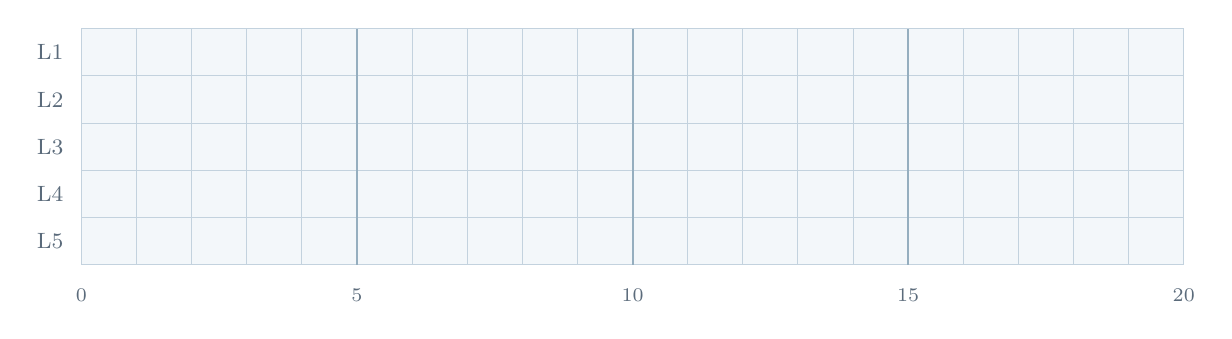
\begin{tikzpicture}[x=0.70cm, y=0.60cm]
  % 5 行 × 20 列网格
  \foreach \r in {0,...,4}{%
    \foreach \c in {1,...,20}{%
      \draw[draw=line, line width=0.35pt, fill=paper]
        (\c-1,\r) rectangle (\c,\r+1);}}
  % 每 5 格加粗分隔
  \foreach \c in {5,10,15}{%
    \draw[main!45, line width=0.7pt] (\c,0) -- (\c,5);}
  % 行标（自上而下 L1–L5）
  \foreach \lab/\yy in {1/4.5, 2/3.5, 3/2.5, 4/1.5, 5/0.5}{%
    \node[anchor=east, font=\footnotesize, text=graytext] at (-0.15,\yy) {L\lab};}
  % 列标（每 5 格）
  \foreach \c/\t in {0/0, 5/5, 10/10, 15/15, 20/20}{%
    \node[font=\scriptsize, text=graytext, anchor=north] at (\c,-0.3) {\t};}
\end{tikzpicture}
\end{center}

\vspace{1.4ex}
{\small\heiti\color{main}二、词汇量刻度尺}
\hspace{0.4em}{\footnotesize\color{graytext}在轴上标出估算词汇量（用三角符号或涂色标出）}\par
\vspace{1.4mm}
\begin{center}
\begin{tikzpicture}[x=0.0066cm, y=0.11cm]
  % 级别色带
  \fill[lvA!25] (0,-1) rectangle (450,-7);
  \fill[lvB!25] (450,-1) rectangle (950,-7);
  \fill[lvC!25] (950,-1) rectangle (1450,-7);
  \fill[lvD!25] (1450,-1) rectangle (1900,-7);
  \fill[lvE!25] (1900,-1) rectangle (2400,-7);
  \node[font=\scriptsize, text=main] at (225,-4) {L1};
  \node[font=\scriptsize, text=main] at (700,-4) {L2};
  \node[font=\scriptsize, text=main] at (1200,-4) {L3};
  \node[font=\scriptsize, text=main] at (1675,-4) {L4};
  \node[font=\scriptsize, text=main] at (2150,-4) {L5};
  % 主轴线
  \draw[main!70, line width=0.9pt] (0,0) -- (2400,0);
  % 刻度
  \foreach \v in {0,200,...,2400}{%
    \draw[main!55, line width=0.4pt] (\v,0) -- (\v,6);}
  \foreach \v in {0,600,1200,1800,2400}{%
    \draw[main!75, line width=0.7pt] (\v,0) -- (\v,10);%
    \node[above, font=\scriptsize, text=graytext] at (\v,10) {\v};}
  % 课标参考线
  \draw[accent, dashed, line width=0.7pt] (1600,-7) -- (1600,12);
  \node[above, font=\scriptsize, text=accent] at (1600,12) {课标 1600 词};
\end{tikzpicture}
\end{center}

\vspace{2.2mm}
\begin{tabularx}{\linewidth}{@{}>{\raggedright\arraybackslash}p{2.2cm}
    >{\raggedright\arraybackslash}X
    >{\raggedright\arraybackslash}p{2.2cm}
    >{\raggedright\arraybackslash}X@{}}
{\small\bfseries 本学期目标} & \fillin[2.6cm] & {\small\bfseries 复测日期} & \fillin[2.6cm]\\[1.1ex]
{\small\bfseries 教师签字} & \fillin[2.6cm] & {\small\bfseries 家长签字} & \fillin[2.6cm]\\[1.1ex]
{\small\bfseries 备\qquad 注} & \multicolumn{3}{l@{}}{\fillin[9.4cm]}
\end{tabularx}
\end{tcolorbox}

\vspace{0.8ex}
\begin{tcolorbox}[softbox]
{\footnotesize\color{graytext}
 \textbf{编制说明}：本单按成都市现行人教版《英语》（2024 新版）初中各册单词表抽样编制，
 5 级 × 20 词，共 100 词；采用“分级通过＋增量估算”定级，抽样误差约 ±10\%，
 用于分层教学与词汇回补，不替代标准化测评。
 \textbf{版本}：升级版 v2.0（2026-10）；可自由复印用于班级教学，请保留本说明。}
\end{tcolorbox}

\end{document}
